\documentclass[12pt]{article}
%\documentclass{moderncv}
%\moderncvtheme[blue]{classic}
%\firstname{Shion}
%\familyname{Chen}
%\usepackage{multibib}


\setlength{\topmargin}{-1.5cm}
\setlength{\oddsidemargin}{-0.3cm}
\setlength{\evensidemargin}{-0.3cm}
\setlength{\textwidth}{16.5cm}
\setlength{\textheight}{23cm}
\usepackage[utf8]{inputenc}
%\usepackage{graphicx}
\usepackage[dvipdfmx]{graphicx}
\usepackage{float}
\usepackage{slashed}
\usepackage{caption}
\usepackage{url, braket, setspace}
\usepackage{amsmath,amsthm,amssymb,bm}
\usepackage{hyperref}
\usepackage{xspace}

\usepackage{tgbonum}

\setlength{\abovedisplayskip}{4pt} % upper margin
\setlength{\belowdisplayskip}{8pt}% lower margin

%%%%%%%%%%%%%%% footer
%\usepackage{lipsum} % for filler text
%\usepackage{fancyhdr}
%\pagestyle{fancy}
%\fancyhead{} % clear all header fields
%\renewcommand{\headrulewidth}{0pt} % no line in header area
%\fancyfoot{} % clear all footer fields
%\fancyfoot[LE,RO]{\thepage}           % page number in "outer" position of footer line
%\fancyfoot[RE,LO]{Shion Chen} % other info in "inner" position of footer line



%%%%%%%% reference
\renewcommand{\refname}{Full List of Publication \hrule height 0.5mm depth 1mm width 100mm}
%\usepackage[sorting=none, backend=biber]{biblatex} % load the package
%\addbibresource{publication/testBI} 
%\addbibresource{publication/ILC_calorimeter.bib} 
%\addbibresource{publication/ATLAS} 

%%%%%%%% section
\newcommand{\Section}[1]{\section*{#1}
\addcontentsline{toc}{section}{#1}}
\newcommand{\Subsection}[1]{\subsection*{#1}
\addcontentsline{toc}{subsection}{#1}}
\newcommand{\Subsubsection}[1]{\subsubsection*{#1}
\addcontentsline{toc}{subsubsection}{#1}}

\usepackage{titlesec}
\titleformat{\section}
  {\normalfont\sffamily\Large\bfseries  }
  {\thesection }{1em}{}
\titleformat{\subsection}
  {\normalfont\sffamily \large \bfseries }
  {\thesection}{1em}{}
\titleformat{\subsubsection}
  {\normalfont\sffamily \bfseries }
  {\thesection}{1em}{}

%%%% Alias %%%%%
\def \mm#1{\mathrm{#1}}
% fig 
\newcommand{\fig}[4][width=15cm]{
\begin{figure}[H]
 \centering
 \includegraphics[width=#1mm]{#2.eps}
 \caption{#3}
 \label{#4}
 \end{figure}} 
%
% Unit
\newcommand{\gev}{\mathrm{GeV}}
\newcommand{\mev}{\mathrm{MeV}}

\newcommand{\ifb}{\ensuremath{\text{fb}^{-1}}\xspace}
\newcommand{\pt}{\ensuremath{p_{\text{T}}}\xspace}
\newcommand{\dm}{\ensuremath{\Delta m}\xspace}
\newcommand{\ra}{\rightarrow}
\newcommand{\GeV}{\text{GeV}\xspace}
\newcommand{\TeV}{\text{TeV}\xspace}

%
%%%%%%%%%%%%
\begin{document}
%\lipsum[1-20] % generate about 4 pages of filler text

\begin{center}
  \large{\textbf{Shion Chen  - {\it Curriculum Vitae}   }} \\
  \vspace{2mm}
  \small{Last update: \today} 
\end{center}

%%%%%%%%%%%%%%%%%%%%%%% Basic info %%%%%%%%%%%%%%%%%%%%%%%
\begin{minipage}[t]{.8\textwidth}
%  \begin{center}
    \begin{tabular}{ll}
      Date of birth: & 17 June 1989 \\
      Nationality: & Japan \\
      Address: & International Center for Elementary Particle \\ 
               & Physics (ICEPP), The University of Tokyo. \\
               & 7-3-1 Hongo Setagaya-ku Tokyo Japan. \\
      email: &  chen@icepp.s.u-tokyo.ac.jp \\
      phone: & +81-3-5841-8384 \\
    \end{tabular}
%  \end{center}
%    \caption*{}
\end{minipage}
  %
\hfill
  %
\begin{minipage}[c]{.15\textwidth}
  \begin{figure}[H]
%    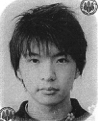
\includegraphics{psp_photo_2010.jpg}
    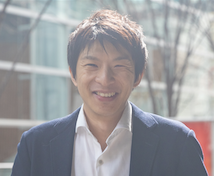
\includegraphics{photo_for_job.png}
  \end{figure}
\end{minipage}


%%%%%%%%%%%%%%%%%%%%%%% Education and Training %%%%%%%%%%%%%%%%%%%%%%%
\Section{Education and Training \hrule height 0.5mm depth 1mm width 100mm}  \vspace{-5mm}
\begin{description}
	 \item[\underline{2014-2017}]   \mbox{}\\
	 	Doctor of Philosophy~(Science), The University of Tokyo, Japan. JPS fellowship~(DC1). \\
      	        Thesis: ``Search for Gluinos using Final States with One Isolated Lepton in the LHC-ATLAS Experiment''. \\
                Advisor: Sachio Komamiya, Shoji Asai.
	 \item[\underline{2012-2014}]  	\mbox{}\\
	 	Master's degree in Physics, The University of Tokyo, Japan.  \\ 
      	        Thesis: ``Test of Bell's Inequality and Entanglement Measurement in Collider Experiments". \\
                Advisor: Sachio Komamiya.
\end{description}

%%%%%%%%%%%%%%%%%%%%%%% Work experience %%%%%%%%%%%%%%%%%%%%%%%
\Section{Work Experience \hrule height 0.5mm depth 1mm width 100mm} \vspace{-5mm}
\begin{description}
	 \item[Project Assistant Professor] (University of Tokyo, Jan 2022-present) \mbox{} \\
               Quantum device development and the application to fundamental physics. \\
	 \item[Post-doctoral fellow] (University of Pennsylvania, Sep 2017-Dec 2021) \mbox{} \\
               Searches for Super-symmetric particle, new lepton tagger development and the operation of the Transition Radiation Tracker in ATLAS experiment. \\
	       Advisor: Brig Williams, Joseph Kroll.               
\end{description}
\clearpage


%%%%%%%%%%%%%%%%%%%%%%% Publication %%%%%%%%%%%%%%%%%%%%%%%
\Section{Selected publications \hrule height 0.5mm depth 1mm width 100mm}  \vspace{-5mm}
\begin{enumerate}
	\item \underline{\textbf{S.~Chen}}, Y.~Nakaguchi and S.~Komamiya \\
			``Testing Bell's Inequality using Charmonium Decays''  \\
			Prog. Theor. Exp. Phys. 063A01 (2013) \label{Pub::BI2013_PTEP}
                         arXiv:~\href{https://arxiv.org/abs/1302.6438}{[hep-ph]~1302.6438}
%
%	\item C.Kozakai, \underline{\textbf{S.Chen}} et.al. (1404.0124)	\\
%          ``Robustness of a SiECAL used in Particle Flow Reconstruction'' \\
%	  International Workshop on Future Linear Colliders (LCWS13) Tokyo, Japan, November 11-15, 2013. \label{Pub::ECAL_LCWS2013} \href{https://arxiv.org/abs/1404.0124}{arXiv:~1404.0124}.
%
%        \item M. S. Amjad, \dots \underline{\textbf{S.Chen}} et al. \\
%              ``Beam test performance of the SKIROC2 ASIC'' \\
%                Nucl. Instrum. Meth., A778:78\UTF{2013}84 (2015) \label{Pub:SKIROC2015}
%
	\item ATLAS Collaboration  \dots \underline{\textbf{S.~Chen}} \dots \\
		   ``Search for gluinos in events with an isolated lepton, jets and missing transverse momentum at $\sqrt{s}= 13$ TeV with the ATLAS detector.'' \\
	             Eur. Phys. J., C 76(10) 565 (2016)    arXiv:~\href{https://arxiv.org/abs/1605.04285}{[hep-ex]~1605.04285} \\
		   ``Search for squarks and gluinos in events with an isolated lepton, jets and missing transverse momentum at $\sqrt{s}=13$ TeV with the ATLAS detector.'' \\
		    Phys. Rev. D 96 112010 (2017)      arXiv:~\href{https://arxiv.org/abs/1708.08232}{[hep-ex]~1708.08232}  \label{Pub::ATLPaper_Incl1L}
%
%  	\item ATLAS Collaboration \dots \underline{\textbf{S. Chen}} \dots \\ 
%		   ``Search for squarks and gluinos in events with an isolated lepton, jets and missing transverse momentum at $\sqrt{s} = 13$ TeV with the ATLAS detector."
%	            ATLAS-CONF-2016-054, 2016. \label{Pub::ATLCONF_Incl1L_ICHEP2016} 
%
%	\item ATLAS Collaboration \dots \underline{\textbf{S. Chen}} \dots \\
%		   ``Search for supersymmetry with two and three leptons and missing transverse momentum in the final state at $\sqrt{s}=13$ TeV with the ATLAS detector."
%		    \href{https://cds.cern.ch/record/2212162}{ATLAS-CONF-2016-096} (2016) \label{Pub::ATLCONF_EW_SEARCH2016}
%
	\item ATLAS Collaboration \dots \underline{\textbf{S. Chen}} \dots \\
		   ``Searches for electroweak production of supersymmetric particles with compressed mass spectra in $\sqrt{s}=13$~TeV $pp$ collisions with the ATLAS detector'' \\
	            Phys. Rev. D 101 052005 (2020) arXiv:~\href{https://arxiv.org/abs/1911.12606}{[hep-ex]~1911.12606}  \label{Pub::ATLPaper_EWCompressed}
%
	\item ATLAS Collaboration \dots \underline{\textbf{S.~Chen}} \dots \\
          ``Search for chargino-neutralino pair production in final states with three leptons and missing transverse momentum in $\sqrt{s}=13$ TeV p-p collisions with the ATLAS detector'' \\
%           \href{https://cds.cern.ch/record/2719521}{ATLAS-CONF-2020-015} (2020)  	\label{Pub::ATLCONT_EW3L_LHCP2020}          
	    Eur. Phys. J. C 81 1118 (2021)  arXiv:~\href{https://arxiv.org/abs/2106.01676}{[hep-ex]~2106.01676}  \label{Pub::ATLPaper_EW3L}
%
	\item ATLAS Collaboration \dots \underline{\textbf{S.~Chen}} \dots \\
          ``Search for charginos and neutralinos in final states with two boosted hadronically decaying bosons and missing transverse momentum in $pp$ collisions at $\sqrt{s}=13$ TeV with the ATLAS detector'' \\
%           \href{https://atlas.web.cern.ch/Atlas/GROUPS/PHYSICS/CONFNOTES/ATLAS-CONF-2021-022/}{ATLAS-CONF-2021-022} (2021)  	\label{Pub::ATLCONF_EW0L_LHCP2021}
	    Phys. Rev. D 104 112010 (2021)  arXiv:~\href{https://arxiv.org/abs/2108.07586}{[hep-ex]~2108.07586}   \label{Pub::ATLPaper_EW0L}          
%
	\item ATLAS Collaboration \dots \underline{\textbf{S.~Chen}} \dots \\
              ``Muon reconstruction and identification efficiency in ATLAS using the full Run 2 $pp$ collision data set at $\sqrt{s}=13$ TeV'' \\
          Eur. Phys. J. C 81 578 (2021) arXiv:~\href{https://arxiv.org/abs/2012.00578}{[hep-ex]~2012.00578}. \label{Pub::ATLPaper_muon_Run2}
%
	\item ATLAS Collaboration \dots \underline{\textbf{S.~Chen}} \dots \\
              ``Radiation effects in the LHC experiments: Impact on detector performance and operation'' \\ 
          CERN Yellow Reports, DOI: \href{https://e-publishing.cern.ch/index.php/CYRM/issue/view/129}{10.23731/CYRM-2021-001}. \label{Pub::CERN_YR_radiation}
%
	\item S.~Chen, H.~Fukuda, T.~Inada, \underline{T.~Moroi}, T.~Nitta and T.~Sichanugrist \\
          ``Detection of hidden photon dark matter using the direct excitation of transmon qubits'' \\
	    Phys. Rev. Lett. 131, 211001 (2023)  arXiv:~\href{https://arxiv.org/abs/2212.03884}{[hep-ex]~2212.03884}   \label{Pub::DMQubits1}
%
	\item S.~Chen, H.~Fukuda, T.~Inada, T.~Moroi, T.~Nitta and \underline{T.~Sichanugrist} \\
          ``Quantum Enhancement in Dark Matter Detection with Quantum Computation'' \\
	    arXiv:~\href{https://arxiv.org/abs/2311.10413}{[hep-ex]~2311.10413}   \label{Pub::DMQubits2}
\end{enumerate}


%%%%%%%%%%%%%%%%%%%%%%% Talks at Confereces %%%%%%%%%%%%%%%%%%%%%%%
\clearpage
\Section{Selected Talks at Conferences \hrule height 0.5mm depth 1mm width 100mm} \vspace{-5mm}
\begin{enumerate}
\item  ``Testing Quantum Mechanics in Collider Experiments'', International School of Sub-nuclear Physics 2015, July 2015, Erice, Italy. \label{Talk:ERICE2015}
%\item ``Test beam analysis of SiW ECAL physics prototype in 2011 FNAL''. CALICE Collaboration Meeting, LAPP, Annecy, France, 2013. \label{Talk:CALICE2013_FNALTB}
%\item Simulation Study on SiW ECAL optimization. In CALICE Collaboration Meeting, LAPP, Annecy, France., 2013.
%\item ``Test of Power Pulsing with the HBU-LED System''. CALICE Collaboration Meeting, LAPP, Annecy, France, 2013. \label{Talk:CALICE2013_PPHBU}
%\item ``A new background suppression technique for LHC-ATLAS Run2 Electroweak Gaugino search'',  Japan physics society meeting, September 2015, Osaka Japan.
%\item ``Search for gluinos in events with a isolated lepton, jets and missing transverse momentum at LHC-ATLAS experiment (2)",  Japan physics society meeting, March 2016, Sendai Japan.
%\item ``Search for super-symmetric particles in one lepton final state in the LHC-ATLAS experiment Run2.'',  Japan physics society meeting, September 2016, Miyazaki Japan.
\item  ``Searches for squarks and gluinos in final states with an isolated charged lepton, jets, and missing transverse momentum with the ATLAS detector'', Epiphany 2017, January 2017, Krakow, Poland. 
\item  ``Electroweak Production SUSY Searches in the ATLAS Experiment'', LHCP 2018, June 2018, Bolonga, Italy. 
\item  ``Search for electroweak gauginos in compressed mass spectra in the LHC-ATLAS experiment'', DPF 2019, July 2019, Boston, USA.  
\item  ``Reconstruction Techniques in SUSY Searches with Soft Objects in the ATLAS Experiment'', ICHEP 2020, July 2020, Prague, Czeck Republic (Remote). 
\item  ``SUSY Searches at LHC'', La Thuile 2022, March 2022, Aosta, Italy. 
\item  ``Dark matter search at LHC: SUSY dark matter'', Kashiwa Dark matter Symposium 2022, November 2022, Kashiwa, Japan. 
\end{enumerate}

%%%%%%%%%%%%%%%%%%%%%%% Seminars %%%%%%%%%%%%%%%%%%%%%%%
\Section{Selected Seminar Talks \hrule height 0.5mm depth 1mm width 100mm}  \vspace{-5mm}
\begin{enumerate}
\item ``Testing Bell's Inequality in the Charm Factory", Shion Chen, Open Seminar talk, 2 December 2013, IHEP, China.
\item ``Testing Bell's Inequality using Momentum-entangled States in Collider Experiments", Shion Chen, KEK theory seminar, 16 December 2013, KEK, Japan.
\item ``Search for electroweak and long-lived SUSY signatures at LHC Run2", Workshop for Tera-scale physics, 23 December 2015, Tokyo Institute of Technology, Japan. 
\item ``Quest for gauginos in LHC-Run2 / ATLAS", Experimental Particle Physics Seminars, 23 December 2016 , University of Pennsylvania, USA. 
\item ``High-lights of SUSY searches at LHC Run2", Workshop for Tera-scale physics, 27 July 2018 , Nagoya University, Japan. 
\item ``Search for gluinos using the 1-lepton final state in the LHC-ATLAS experiment", Japan Physics society, 15 March 2019, Kyushu University, Japan. 
\end{enumerate}

%%%%%%%%%%%%%%%%%%%%%%% Grants & Awards %%%%%%%%%%%%%%%%%%%%%%%
\clearpage
\Section{Research Grants and Awards \hrule height 0.5mm depth 1mm width 100mm} \vspace{-5mm}
\begin{enumerate}
\item DESY summer student project (2013). 
\item Research Fellow (DC1), Japan Society for the Promotion of Science (April 2014 - 2017).
%\item ``Best Science Secretariat Award", International School of Sub-nuclear Physics 2015 (July 2015, Erice, Italy).
\item CERN relay race, 2nd place, as member of Tokyo HipHoppers  (21 May 2015 CERN, Switzerland).
%\item CERN relay race, 3rd place, as member of Tokyo HipHoppers (19 May 2016 CERN, Switzerland).
\item  \href{https://www.jps.or.jp/english/file/13th_wakate2019.pdf}{Young scientist award, Japan Physics Society (2019).}
\item \href{https://cds.cern.ch/record/2752244}{ATLAS Outstanding Achievement Award (2021)} \\
On the outstanding contributions to the DAQ upgrades directed to the TRT operation at high occupancy and trigger rate.'
\end{enumerate}

%%%%%%%%%%%%%%%%%%%%%%% Languages %%%%%%%%%%%%%%%%%%%%%%%
\Section{Languages \hrule height 0.5mm depth 1mm width 80mm} \vspace{-5mm}
Japanese (native), Mandarin Chinese (native), English (fluent), French (decent), Brasilian Portuguese (awful).

%\clearpage 
\Section{Research Summary \hrule height 0.5mm depth 1mm width 100mm} \vspace{-5mm}
(All the references cited in the section correspond to the numbering in the ``Selected Publication" above.) \\

My research career has been driven by a simple desire of understanding the fundamental rules of the nature. 
For the five years as a graduate student in The University of Tokyo, and three years as a postdoc in University of Pennsylvania, 
I have pursued the fundamental theories of quantum mechanics and elementary particle physics using the platform of high energy physics, or sometimes vice versa.
The topics include:
\begin{itemize}		
\item Phenomenological analyses of quantum entanglement in the multi-body systems realized in collider experiments,
\item Development of calorimeters for the future international linear collider (ILC) project,
\item Searches for supersymmetry in the ATLAS experiment in the energy frontier Large Hadron Collider (LHC) at CERN,
\item Quantum device development and the application to wave-like dark matter searches.
\end{itemize}	

%%%%%%%%%%%%%%%%%%%%%%%%%%%%%% Quantum %%%%%%%%%%%%%%%%%%%%%%%%%%%%%%%
\Subsection{Quantum device development and Wave-like dark matter searches using superconducting qubits (2022-present) \hrule height 0.1mm depth 0.1mm width 165mm}
Since 2022 moving back to ICEPP/UTokyo, I also joined the looming quantum hardware team in the institute.
The scope spans from developing quantum devices in the context of the superconducting NISQ computers, 
high-Q cavity application for quantum memory or transduction,
to introduction of qubits to the next generation haloscope experiments targeting wave-like dark matter such as dark photon or axion.
The initiation efforts include establishing the fabrication of the own superconducting qubits and the peripheral devices (cavities, PCBs etc.),
as well as setting up the low-temperature measurement testbed located in the Mili-kelvin Quantum Platform of Cryogenic Research Center at The University of Tokyo. 
These are achieved within a year: a transmon qubit of $T_1 \sim 10~\mu \text{s}$ has been already fabricated and confirmed in the cryogenic testbed. \\

A new wave-like dark matter search scheme using the superconducting qubits are also devised 
in a collaboration with the phenomenologiest colleagues in the department~[\ref{Pub::DMQubits1}].
This is to use the ac E-field induced by the dark photon dark matter as the ``drive field'' for the qubits,
and observe the slow yet coherent excitation as the signal.
The key element of the scheme is to utilize the large electric dipole moment of the qubits.
The strong coupling allows to detect very feeble electric field, achieving a promising sensitivity.
The easy frequency tunability of the qubits also enables the mass scan without significant engineering efforts, 
which is remarkable considering the struggle of the other experiments targeting the similar mass regime.
The experiment is currently under preparation. The data taking is expected to start in early 2023.

%%%%%%%%%%%%%%%%%%%%%%%%%%%%%% ATLAS %%%%%%%%%%%%%%%%%%%%%%%%%%%%%%%
\Subsection{ATLAS experiment  (2014-present) \hrule height 0.1mm depth 0.1mm width 165mm}

%%%%%%%%%%%%%%
\paragraph{Operation and Upgrades of the TRT Detector (2017-2021)} \phantom{k} \vspace{2mm} \\
Transition Radiation Tracker (TRT) is one of the primary tracking detectors in the ATLAS.
It consists of 350,848 cylindrical 4~mm diameter straws of thin-wall proportional chamber filled with Xe/Ar-based active gas, 
creating ionization signals along a passage of a charged particle.
While it serves as a continuous tracker, it also offers a particle identification functionality 
via the transition radiation radiated emitted from the polyethylene fiber/foils interspaced between the straws. \\

Since April 2017 I have been part of the DAQ operation crew of the TRT as a member of University of Pennsylvania,
and have served as the DAQ coordinator since August 2018.
The main responsibility is to ensure the smooth data-taking -- from continual calibrations of low-voltage setting on front-end electronics, threshold setting, and fine delay setting,
to the data flow handling from the front-end, monitoring, recovery during the operation and so on.
The year of 2017 was particularly challenging for the TRT DAQ as the LHC decided to exceed the design goal in its luminosity. 
As having providing almost two times higher instantaneous luminosity than the nominal value, it saturated the bandwidth in many different parts of the read out path.
Numerous DAQ upgrades were implemented since 2016 that includes refining the data format sent off the front-end, 
over-clocking the back-end electronics, 
improving the data compression scheme,
and replacement of the transceiver cards on the back-end electronics board.
I joined from the middle of the upgrades and contributed to the commissioning using the high-luminosity data-taking since the late 2017 operation. \\

Though the upgrades ended with a great success, we started to observe sporadic events of de-synchronization in the detector since the high-luminosity operation in Run2.
While each de-synchronization only costs about 15 seconds of dead time for the auto-recovery, 
it was crucial to understand the root cause since it can develop in the future if it is related to the hardware.
I have been leading the investigation activity since 2018.
The biggest challenge was that this error was never been reproduced in any environments other than the real collisions.
Still, through the in-situ hardware swapping tests and a careful log analysis,
we could almost identify that the Quartz Crystal Based PLL (QPLL) chips on some patch panel boards are the most suspicious components.
Numerous tests are in progress to understand the actual mechanism, and a potential QPLL chip replacement campaign is planned once it is proven. \\

The other activities during the Long Shut-down 2 (LS2; 2019-2022) include the improving the on-line DAQ software, 
upgrade of the Trigger and Timing Controller system, stress-testing of the hardware spares, and the radiation damage assessment in the TRT over the Run1-2~[\ref{Pub::CERN_YR_radiation}]. 
The DAQ team has been awarded for the ATLAS Outstanding Achievement Award for the overall efforts in 2018-20 (see the ``Research Grants and Awards'' above). 

%%%%%%%%%%%%%%
\paragraph{Searches for Electroweakino production (2015-2021)}  \phantom{k} \vspace{3mm} \\
Supersymmetry (SUSY) in the particle physics is an elegant theoretical extension of the Standard Model (SM) 
by introducing new particles that have the identical quantum numbers with the SM partners except for the spins.
While it is generally desirable as the solution of the hierarchy problem and the grand-unification,
light electroweakinos -- the SUSY partners of the SM gauge bosons and the higgs boson -- are particularly well-motivated 
in terms of the presence of viable WIMP dark matter candidate, naturalness, consistency with the potential muon g-2 anomaly and so on. \\

\Subsubsection{First electroweakino search in ATLAS Run2 (2015-2016)}
Due to the small production cross-section,
the production of electroweakinos were only poorly constrained by direct searches before the LHC Run2 when I joined the ATLAS.
As as Ph.D student, I participated to the first chargino-neutralino pair production search in the Run2 using the 3-lepton final state and the datasets corresponding to 14.8\ifb.
%~[\ref{Pub::ATLCONF_EW_SEARCH2016}]. 
The contribution was mainly in the area of event selection optimization and fake lepton estimation based on the vastly improved particle ID performance,
as well as the software development and validation adopting to the new Run2 data format and framework.
Although there was no sign of new physics found and the achieved sensitivity was still limited in that round, 
the analysis strategy and the software legacies were substantially inherited to the later series of the same analysis carried out with larger data statistics. \\

After a year leaving for my graduation and coming back to the SUSY group again as a postdoc, 
I set out tackling two frontiers that limited the search sensitivity: the ``compressed spectra frontier'' and the ``high-mass'' frontier:
%%%%%%
\Subsubsection{Compressed spectra searches in the 2-/3-lepton final states (2018-2021)}
The compressed spectra in SUSY refers to a regime where the mass splitting between the produced SUSY particles and the lightest SUSY particle --LSP-- (\dm) is small, ending up in only soft particles in the final states.
Though this is exceptionally motivated regime by the thermal dark-matter relic density or naturalness,
the search sensitivity faces a harsh challenge in the low-\pt electrons/muons (collectively referred to ``leptons'') reconstruction versus the high fake lepton background from jets,
The best exclusion limit at that time was set only up to $140-180~(90-140)~\GeV$ for wino (higgsino) production for $\dm<100~\GeV$, using the full-Run1 or the Run2 36.1\ifb datasets.
To overcome the limitation, my effort was put on improving the fake rejection by developing a machine-learning based lepton selection algorithm with particular focus on low-\pt leptons (more detailed in the next section)~[\ref{Pub::ATLPaper_muon_Run2}],
understanding the performance, calibrating with data and introduced to the searches using the 2- or 3-lepton final states~[\ref{Pub::ATLPaper_EWCompressed},\ref{Pub::ATLPaper_EW3L}].
Having committed to the both analysis, I have contributed more to the 3-lepton search as one of the main analyzers
devising a new kinematic variable helping the discrimination, 
defining the event triggering strategies, 
polishing the event selections and advising the students in the team on various aspects of the analysis.
Unfortunately again there was no evidence found beyond the SM expectation in the both analyses, 
the exclusion could run up to $\sim 250-300~(150-200)~\GeV$ for the wino (higgsino) production with $3~\GeV<\dm<100~\GeV$ using the full Run2 datasets. 
This corresponds to excluding signals with 5--15 times smaller cross-section with respect to the previous analyses, 
overwhelming the benefit of simply increasing the data statistics. \\
%%%%%%
\Subsubsection{High-mass search using the boosted hadronic final states (2018-2021)}
The high-mass frontier is on the other hand a regime where heavy electroweakinos are produced decaying into a substantially lighter LSP.
Besides the small production cross-section, the bottleneck was identified to be the lepton requirement employed in the analyses (in a fear of being overwhelmed by the high hadronic backgrounds otherwise)
that suppresses the signal yields typically by about the branching ratio of $W \ra \ell\nu$ or $Z \ra \ell\ell$ (1/15-1/4).
To entirely overcome this limitation, I have initiated a new effort targeting fully-hadronic final states exploiting the ``boosted boson tagging'' technique based on the ``large-radius jets'' reconstruction and the discrimination power of the jet substructure information. %~\cite{ATL-PHYS-PUB-2020-017}  
This was the first electroweakino search in the LHC focusing on the final states, as well as one of the few analyses nowadays that targeted the phase space that had been never covered.
The major focus of the studies was on re-optimizing the boson tagging selection and understanding backgrounds, such as the main $W/Z$+jets background with multiple gluon-splitting processes as well as various instrumental backgrounds, which are very uncommon and hard to predict.
Though again no sign beyond the SM prediction was seen, the result could set by far the most stringent constraints excluding unprecedentedly heavy electroweakino up to $\sim 1~\TeV$~($800~\GeV$) for wino (higgsino) pair production in general, when the mass splitting is great than $400~\GeV$. 
This typically compares with the projected exclusion limits at an integrated luminosity of 1-3~ab$^{-1}$ by the convention searches using the other final states.
The analysis also achieved a dramatically small model dependency in the sensitivity thanks to treating the decays of $W/Z/h$ bosons inclusively.
A remarkably wide model interpretation is also provided testing the exclusion of various LSP assumptions (wino, higgsino, bino, gravitino, and axino) and the branching hypotheses,
which enables to declare generic exclusion limits on the electroweakino pair production~[\ref{Pub::ATLPaper_EW0L}].
%\clearpage 

%%%%%%%%%%%%%%
%\Subsubsection{Development and the Calibration of a new Lepton Isolation Algorithm using Machine-Learing (2018-2020)} 
\paragraph{Development and the Calibration of a new Lepton Isolation Algorithm using Machine-Learing (2018-2020)}  \phantom{k} \vspace{3mm} \\
Lepton isolation requirement is a follow-up selection suppressing fake leptons that evade the rejection by the upstream electron/muon identification.
As opposed to the sophisticated multi-variate analysis techniques employed in the other fields of object reconstruction in ATLAS such as the electron ID and b-tagging,
only very simple selections have been exercised in isolation, which are typically the fixed cuts in the energy sum of tracks and calorimeter clusters around the lepton candidate.
In 2016, the first machine-learning based isolation was contrived in the context of $t\bar{t}+h$ search. 
This was a boosted decision tree (BDT) taking eight input variables including number of tracks around the lepton, vectorial sum of those momenta, and $b$-jet likeliness calculated by the $b$-tagging algorithm, 
achieving another factor of 2-4 fake lepton reduction with $70\%-90\%$ real lepton efficiency after applying the standard isolation cut.  \\

While this algorithm was specifically targeting high-\pt ($>30$~GeV) fakes from heavy-flavor hadron decays,
my interest was to extend the algorithm to a broader scope, and particularly develop a ``low-\pt tune'' that could help the compressed SUSY analysis I was working on.
The retuning was done with Shunichi Akatsuka (University of Kyoto) by re-training with special low-\pt samples and re-optimizing the choice of input variables.
This could eventually achieve $\sim 30-50~(15)\%$ more fake reduction at the same efficiency for electrons (muons). \\

The latter part of my effort was to promote the algorithm as the standard in ATLAS.
A couple of working points were defined by smoothly connecting the nominal and the low-\pt tune, and the efficiency measurements were done to provide the correction factors for the MC.
While the data-vs-MC difference is usually more significant than the traditional isolation variables as expected, the source of the discrepancy was carefully investigated, narrowing down to a few input variables, which helped controlling the impact of the discrepancy.
The BDT isolation working points became available as the collaboration-wide recommendation since 2020~[\ref{Pub::ATLPaper_muon_Run2}].


%%%%%%%%%%%%%%
%\Subsubsection{Search for Gluino production using the 1-lepton final state (2015-17)} 
\paragraph{Search for Gluino production using the 1-lepton final state (2015-2017)}  \phantom{k} \vspace{3mm} \\
Since the discovery of higgs boson at a mass of 125 GeV, there is a dramatically increased interest in the search for gauginos since in typical minimal models, this mass naively implies a scalar top mass of several tens of TeV, beyond the reach of LHC. In the early stage of LHC Run2, the gluino search was particularly well-motivated as its production cross-section increases by a factor 4-40 due to the doubled center of mass energy with respect to Run1. \\

As the dissertation analysis, I participated in a gluino search focusing on the final state with exactly one lepton. 
My major contribution to this analysis was in the background estimation. 
While a careful and dedicated background modeling is crucial for a discovery-oriented analysis, 
it is challenging in this analysis because the signal region lies in the high energy tails of SM phase space. 
The background remaining after the selection are very unusual events, 
typically associated with many jets generated at higher-order QCD.
Therefore the MC-based estimation -- even assisted by the use of control regions laying in the vicinity of the signal regions -- may not be always reliable.
Half of the background events in the signal regions also arises from di-lepton events where one of the leptons are mis-identified or a tau lepton decays hadronically, faking as a jet.
To address the estimation on this background component, I have developed a new data-driven estimation method that uses events with two leptons, 
replacing one of them into a missing particle or a simulated hadronically decaying tau
in order to emulate the events in the signal regions.
Though the achieved precision is still comparable with the nominal method, the new method significantly reduce the reliance on the MC, adding robustness to the estimation.
On the other hand, I have also worked on investigating the MC mis-modeling of several main SM processes in the physics modeling group.
Two results were published from the analysis with different data statistics~[\ref{Pub::ATLPaper_Incl1L}]. 
Unfortunately no significant deviation from the SM was observed, and an exclusion limit was set in a simplified model in which the gluino decays via a chargino.
Up to a gluino mass of 1.7--2.0~TeV was excluded for LSP light than $\sim1$~TeV. 

%\Subsubsection{Development of a databasing system for the MicroMegas detector (2014-15)} 
\paragraph{Development of a databasing system for the MicroMegas detector (2014-2015)}  \phantom{k} \vspace{1mm} \\
MicroMegas is a sub-detector of the New Small Wheel, aiming fast and precise measurements of muon tracks oriented to the end-caps. 
After a successful  R$\&$D and a proposal with TDR, it is now at the stage of fine-tuning the detailed design, 
including the geometry and electronics and so on. 
Simulation studies in accurate geometry therefore became highly important. 
As my authorship qualification project in ATLAS, I developed a centralized database storing the up-to-date geometrical parameters that are sufficient to define whole active area of MicroMegas in simulation.  \\ \\
%%%%%%%%%%%%

%%%%%%%%%%%%%%%%%%%%%%% ILC %%%%%%%%%%%%%%%%%%%%%%%%%%%%
\Subsection{Calorimeter developments for ILC/ILD  (2012-2014) \hrule height 0.1mm depth 0.1mm width 165mm} 
The ILC (International Linear Collider) is a  (sub)TeV-scale electron-positron collider aiming precision measurements of the higgs boson, 
as well as probing new physics in the electroweak sector.  
As targeted events typically contain electroweak gauge bosons (W/Z), 
the precise identification, particularly through their hadronic decay mode, is crucial for many of the ILC physics programs. 
The requirement from physics is sub-5\% energy resolution per jet, which is equivalent to 3-4 GeV resolution for di-jet invariant mass. 
To achieve this unprecedented benchmark, the ILD (International Large Detector) is planning to employ the particle flow algorithm (PFA) 
in which each jet particle is identified and the energy is measured individually. 
The calorimeters are the key components in this regime in which resolving the showers inside jets is key to the performance. \\
%in which jet particles are classified into charged or neutral particles, and the energy measured by the inner tracker or by the calorimeter is assigned for respective type. This realizes the best resolution and correct scale assignment for each individual particle. Successful association of charged tracks and calorimeter deposits is the key part of the algorithm, even in a dense environment crowded with tens of particles per jet. Therefore a highly granular spatial segmentation is required for the ILD calorimeters. \\
%%%% ??????

During the second half of my master course, I participated in the development of the silicon-tungsten electromagnetic calorimeter (SiW-ECAL) and analogue hadronic calorimeter (AHCAL) in the CALICE Collaboration for the ILD. \\

%%%%%%%%%%%%%
%\Subsubsection{Commissioning of the ILD SiW-ECAL prototypes (2013)}
\paragraph{Commissioning of the ILD SiW-ECAL prototypes (2013)}  \phantom{k} \vspace{3mm} \\
To resolve individual clusters inside jets, a highly granular spatial segmentation is required for ILD calorimeters. 
A silicon-tungsten sampling calorimeter is the one of the leading candidate technology for the ILD electromagnetic calorimeter where the silicon sensor layers are segmented into 5-10mm pixels. 
The first generation prototype, with about 10000 readout channels, was developed in the CALICE collaboration in 2006, and regularly tested in test beam experiments since then. 
I analyzed the data collected at a test beam in FNAL in 2011, and verified that the basic performance (linearity, energy resolution, spatial resolution of cluster centeroid etc.) fulfills the requirements. 
The second-generation prototype was designed as a test for a fully integrated detector including data acquisition system with newly developed readout ASICs (SKIROC2).%~[\ref{Pub:SKIROC2015}]. 

%%%%%%%%%%%%%
%\Subsubsection{Study on performance of PFA/ILD SiW-ECAL in a realistic detector setup   (2012-14)} 
\paragraph{Performance study of the PFA/ILD SiW-ECAL in a realistic detector setup   (2012-2014)}  \phantom{k} \vspace{3mm} \\
While simulation studies have shown that PFA with the ideal ILD detector model performs very successfully, 
there are still a number of industrial challenges to achieve the specification of an ideal detector with ideal digitization, 
for instance the increased dead volume due to realistic PCB thickness or the protection frames around silicon sensor cells (``guard ring") which did not present in the baseline simulation model.
%For instance, in the ECAL, It is reportedly hard to to manufacture PCBs with sufficient mechanical strength and robustness within the designed thickness (0.5mm), therefore in a realistic detector thicker volume of PCBs has to be taken into account. Also for SiW-ECAL, in order to suppress noise originated from dark current on the surface of silicon sensors, placing a metal rings around a sensor (``guard ring") has been suggested, which however results in dead volume. \\
I performed a set of studies on the impact of such effects due to the features of a realistic detector on physics performance. 
The jet energy scale and resolution were parametrized as a function of guard ring width,
PCB thickness, fraction of dead pixels/ASICs, noise rate, and cross-talk rate between channels etc., 
and closely evaluated the dependency using simulation. 
The results illustrate that the performance of PFA even under the most pessimistic conditions is still excellent and robust, %~[\ref{Pub::ECAL_LCWS2013}], 
and also provides primary guidance for the definition of manufacturing requirements in the future. 

%%%%%%%%%%%%%
%\Subsubsection{Commissioning of the power-pulsing scheme for ILD AHCAL (2013)} 
\paragraph{Commissioning of the power-pulsing scheme for ILD AHCAL (2013)}  \phantom{k} \vspace{3mm} \\
Due to the beam structure in ILC (1ms of beam out of a 200ms long cycle), 
a power cycling scheme called ``power-pulsing" has been proposed to minimize the power consumption of the detector. 
In this scheme, the power supply is synchronized with the beams so that the power is turned off when the collisions do not take place. 
The DESY FLC group has been working on implementing this into the AHCAL electronics. 
In 2013, I joined the commissioning using the test board as my summer student project at DESY. \\

The test board consists of a detector layer instrumented with 30~mm $\times$ 30~mm square cells of plastic scintillator each equipped with a SiPM, 
and a readout layer with the front-end electronics interfaced to the SiPM attached on the back. 
The tests were performed by injecting the LED pulses, and investigate the response of the readout cycle of the detector in the time domain using a realistic setup. 
Some unstable behavior was observed shortly after turning on the electronics, 
such as worsened resolution in the single photon spectra from the SiPM as well as the gain drop. 
I have evaluated the impact on the data quality and measured the relaxation time of the behavior, 
as well as seeking the optimal board configuration to mitigate the effects. \\

%\clearpage


%%%%%%%%%%%%%%  BI   %%%%%%%%%%%%%%%%%%%%%%%%%%%%
\Subsection{Testing local-reality in collider experiments  (2012-2014) \hrule height 0.1mm depth 0.1mm width 165mm}
Quantum mechanics (QM) is without doubt a very successful theoretical framework in describing physics of the microscopic scale, 
however it is seemingly still on a non-trivial basis; whether observables are intrinsically indeterministic (``non-realism'') and whether the nature can be ``non-local''. 
Such counter-intuitiveness in fact faced various skepticism as articulated by the ``EPR paradox''.
While this had been considered rather as a philosophical problem about the ``picture'' for a long time, 
J.~S.~Bell revealed that there was a phenomenological difference between the quantum and classical (local-realism) pictures through Bell's inequality
i.e. now that this is a scientific problem testable by experiments.
The violation was convincingly concluded by the experiments in 1980s using entangled photon pairs, which eloquently indicated the exclusion of the local-realism.
Although loopholes were pointed out in the early experiments, these have been dramatically improved thanks to the rapid evolution of photon sensing and the laser technology. 
It is finally the time we have to say goodbye to our intuitive -- local and deterministic -- picture of physics.  \\
%The exclusion of local-realism has become almost complete in the photon pair regime, and nowadays nobody views it as paradox anymore. \\

So anything still left to do in the post-EPR era? Yes -- experiments in the other kind of systems are also interesting in terms of testing the universality of quantum nature. 
In particular, tests of Bell's inequality using entangled massive particles are non-trivial as they are more 'classical' due to its shorter Compton wavelength. 
Few experiments were done so far, due to the technical difficulties of preparing and measuring the entangled states. 
High energy colliders have been anticipated as a new platform,
since spin-entangled particle pairs can be easily prepared via a variety of processes with large statistics, 
in a wide range of energies from a few GeV to an order of a few 100~GeV, 
and with various types of interaction involved. 
The spin can be then measured by reconstructing the decay angle distribution of the decay products.
The down-side is the nature of indirect measurements i.e. the spin can only be measured through its decay to which observer's free-will cannot intervene (``free-will loophole'').
Nevertheless it can open up a various available channels even though at some cost of rigorousness. \\

My master thesis project was to study the feasibility i.e. what particle systems are ideal and how statistically significant those channels can be.
This compelled reformulating Bell's inequality for the particular problem, and we obtained a brief metric for the level of violation~[\ref{Pub::BI2013_PTEP}]. 
Checking in the past and ongoing experiments, charmonium decays ($J/\psi,\eta_c^0, \chi_c^0 \ra \Lambda \overline{\Lambda}$) in BES3, 
the di-tau production at Belle ($ee \ra \tau\tau$) and $H\rightarrow \tau\tau$ in ILC are statistically promising with $2-3\sigma$ level of significance. 
Finally, the effect of detector resolution and the background contamination is discussed along with the possible loopholes arising from the setup.
%
%
%%%%%%%%%%%%%%%% Full list of publicatoin %%%%%%%%%%%%%%%%%%%%%%%%%%%%%%%%%%%%%%%%%

%\bibliographystyle{plain}
%\bibliography{publication/nonATLAS}  
%\nocite{*}

%\bibliographystyle{unsrt}
%\bibliography{publication/pub}  


%\clearpage

%\bibliographystyle{unsrt}
%\nocite{*}
%\bibliography{publication/pub}  

\if 0
\Section{Full List of Publication \hrule height 0.5mm depth 1mm width 100mm}
\Subsection{Testing local-reality in collider experiments.  (2012-2013) \hrule height 0.1mm depth 0.1mm width 165mm}
%\bibliographystyle{unsrt}    
%\nocite{*}
cite \cite{Chen:2013epa}
\begin{refsection}[publication/testBI]
\printbibliography[heading=subbibliography] % print section bibliography
\end{refsection}

%\Subsection{Development of calorimeters for ILC/ILD  (2012-2014) \hrule height 0.1mm depth 0.1mm width 165mm} 
%\include{fullPub_ILC}
\fi




\end{document}
